\documentclass[../calc1-main.tex]{subfiles}

\begin{document}
  A \textbf{function} $f$ on a set $D$ (called the \textbf{domain}) into a set $R$ (called the target or codomain) is a rule that assigns a unique element $f(x)$ in $R$ to \textit{each} element $x$ in $D$.

  The \textbf{range} of $f$ is a subset of $R$ containing of all possible values $f(x)$. The range set is not necessarily the same as the target set.

  So technically a function is a triple $(f, D, R)$. However, the triple notation is too cumbersome and we will usually call a function by the label of its rule $f$.

  \begin{figure}[H]
    \centering
    \begin{subfigure}{0.3\textwidth}
      \centering
      \begin{tikzpicture}[scale=.8]
  %put some nodes on the left
  \node at (1,5) {A function};
  \foreach \x in {1,2,3}{
  \node[fill,circle,inner sep=2pt] (d\x) at (0,\x) {};
  \node[left] (dt\x) at (0, \x) {$d_{\x}$};
  }

  \node (D) at (-1.5,4) {D};
  \node[fit=(d1) (d2) (d3) (dt1) (dt2) (dt3),ellipse,draw,minimum width=1cm] {};
  %put some nodes on the center
  \foreach \x[count=\xi] in {1,2,3,4}{
  \node[fill,circle,inner sep=2pt] (r\xi) at (2,\x-.5) {};
  \node[right] (rt\x) at (2, \x-.5) {$t_{\x}$};
  }
  \node (S) at (3.5,4) {R};
  \node[fit=(r1) (r2) (r3) (r4) (rt1) (rt2) (rt3) (rt4),ellipse,draw,minimum width=1.5cm] {};
  \draw[-latex] (d1) -- (r2);
  \draw[-latex] (d2) -- (r2);
  \draw[-latex] (d3) -- (r4);
\end{tikzpicture}
    \end{subfigure}
    \begin{subfigure}{0.3\textwidth}
      \centering
      \begin{tikzpicture}[scale=.8]
  \node at (1,5) {Not a function};
%put some nodes on the left
\foreach \x in {1,2,3}{
  \node[fill,circle,inner sep=2pt] (d\x) at (0,\x) {};
}
\node (D) at (-0.5,4) {D};
\node[fit=(d1) (d2) (d3),ellipse,draw,minimum width=1cm] {};
%put some nodes on the center
\foreach \x[count=\xi] in {0.5,1.5,...,4}{
  \node[fill,circle,inner sep=2pt] (r\xi) at (2,\x) {};
}
\node (S) at (3,4) {R};
\node[fit=(r1) (r2) (r3) (r4),ellipse,draw,minimum width=1.5cm] {};
\draw[-latex] (d1) -- (r1);
\draw[-latex] (d2) -- (r2);
\draw[-latex] (d2) -- (r3);
\draw[-latex] (d3) -- (r4);
\end{tikzpicture}
    \end{subfigure}
  \end{figure}

  \begin{example}
    Define a function on the set of all real numbers by $f(x)=x^2+1$. Find $f(0), \, f(2), \, f(x+2)$.
  \end{example}

  In this class, the target set $R$ of a function will almost always be the set of real numbers $\mathbb{R}$. Such functions are called real valued functions.

  In this class, the domain set will always be a subset of real numbers. When defining a function, its domain should be defined. For example,
  \[
    f(x) = \frac{1}{x}, \qquad x > 0
  \]
  means that the domain of $f$ is the set $\{x \mid x > 0\}$. This function is different from the function
  \[
    f(x) = \frac{1}{x}, \qquad x < 0.
  \]

  However we will usually skip writing the domain of a function. When we do this, the \textbf{domain convention} is to assume that the domain of a function is the set of all real numbers for which its rule is defined.

  The domain of the function
  \[
    f(x)=\frac{1}{x},
  \]
  is the set of all real numbers except $0$.


  \begin{example}
    Find the domain of $f(x) = \dfrac{1}{x^2 - x}$.
  \end{example}

% A function $f: D \to R$ is \textbf{1-1} if $f(x_1) = f(x_2)$ then $x_1=x_2$. A function $f: D \to R$ is \textbf{onto} if for every $y \in R$, there is an $x \in D$ such that $f(x) = y$.

% \begin{example}
%   Draw functions which are 1-1, onto, not 1-1 and not onto,  similar to the Figure~\ref{fig:funcNotfunc}.
% \end{example}

\subsection*{Graph of a function}
\begin{quote}
  A picture is worth a thousand words.
\end{quote}

The \emph{graph of a function} $f$ is the set of all points whose coordinates are $(x, f(x))$ where $x$ is in the domain of $f$. We can visualize a function by plotting its graph set on the Cartesian plane.

\begin{quote}
  Why is visualization important? The answer probably lies in human psychology.
\end{quote}

\begin{figure}[H]
  \centering
  \usetikzlibrary{intersections,backgrounds}
\begin{tikzpicture}

\draw [thick,-stealth] (-0.5,0) --node[below]{domain} (4,0) node[below]{$x$};
\draw [thick,-stealth] (0,-0.5) -- (0,3) node[left]{$y$};
\node [below left] at (0,0) {$0$};

\draw [ultra thick, red] (0.5,0) -- (3.5,0);


\coordinate (start) at (0.499,0.7);
\coordinate (stop) at (3.501,2.5);

\fill (start) circle[radius=2pt];
\fill (stop) circle[radius=2pt];
\draw [name path=curve] (start) to[out=-35,in=190] node[pos=0.6,above left] {} (stop);

\foreach \x in {0.5,1,...,3.5}
  {
  \path [name path=line] (\x,0) -- (\x,3);
  \draw [name intersections={of=curve and line},dashed,-stealth]
   (intersection-1) -- (\x,0);
 }


\begin{scope}[xshift=6cm]
\draw [thick,-stealth] (-0.5,0) --  (4,0) node[below]{$x$};
\draw [thick,-stealth] (0,-0.5) --node[left]{range} (0,3) node[left]{$y$};
\node [below left] at (0,0) {$0$};

\draw [ultra thick, red] (0,0.52) -- (0,2.5);

\coordinate (start) at (0.499,0.7);
\coordinate (stop) at (3.501,2.5);

\fill (start) circle[radius=2pt];
\fill (stop) circle[radius=2pt];
\draw [name path=curve] (start) to[out=-40,in=190] node[pos=0.6,below right] {} (stop);

\foreach \y in {0.52,.916,...,2.5}
  {
  \path [name path=line] (0,\y) -- (4,\y);
  \draw [name intersections={of=curve and line},dashed,-stealth]
   (intersection-1) -- (0,\y);
 }

\end{scope}

\end{tikzpicture}
\end{figure}

\subsection*{Some Elementary Functions}

\subsubsection*{Linear Function}
A function which is given by the formula
\[
  f(x) = mx + n
\]
where $m$ and $n$ are constants is called a \textbf{linear function}. Its graph is a straight line. The constants $m$ and $n$ are the \emph{slope} and \emph{$y$-intercept} of the line. Its domain is all $x$ and its range is all $x$.

\begin{figure}[H]
  \centering
  \pgfplotsset{soldot/.style={color=black,only marks,mark=*}}
\pgfplotsset{holdot/.style={color=black,fill=white,only marks,mark=*}}

\begin{tikzpicture}
  \begin{axis}[
  axis lines=middle, % left, right, box, center, none
  x=8mm,
  y=8mm,
  title={$f(x)=mx+n$},
  xlabel=$x$,
  ylabel=$y$,
  xtick={-2,0},
  ytick={1},
  xticklabels={$-\frac{n}{m}$,0},
  yticklabels={$n$}
  ]
  \addplot[domain=-3:3, very thick] {.5*x+1};
  \addplot[soldot] coordinates{(-2,0)(0,1)};
\end{axis}
\end{tikzpicture}
\end{figure}

\subsubsection*{Square Root Function}
The square root function $f(x) = \sqrt{x}$ has domain $[0, \infty)$ and takes $x$ to its positive square root. Hence it has range $[0, \infty)$.

\begin{figure}[H]
  \centering
  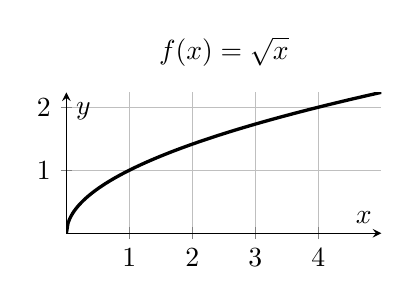
\begin{tikzpicture}
  \begin{axis}[
  axis lines=center, % left, right, box, center, none
  x=8mm,
  y=8mm,
  title={$f(x)=\sqrt{x}$},
  xlabel=$x$,
  ylabel=$y$,
  xtick={1,2,3,4},
  ytick={1,2},
  grid=major,
  ]
  \addplot[domain=0:5, very thick, samples=200] {sqrt(x)};
\end{axis}
\end{tikzpicture}
\end{figure}

\begin{example}
  Find the domain of $f(x) = \sqrt{2-x}$.
\end{example}
\begin{solution}
  Its domain is all $x$ for which $2-x \ge 0$, i.e. the interval $(-\infty, 2]$.
\end{solution}

\subsubsection*{The absolute value function}
The absolute value function is
\[
  \abs{x} =
  \begin{cases}
    x, &\text{ if } x \ge 0\\
    -x, &\text{ if } x < 0
  \end{cases}
\]
Its domain $(-\infty, \infty)$ and range $[0, \infty)$.
We can only define the absolute value function by
$f(x) = \abs{x} = \sqrt{x^2}$.

\begin{figure}[H]
  \centering
  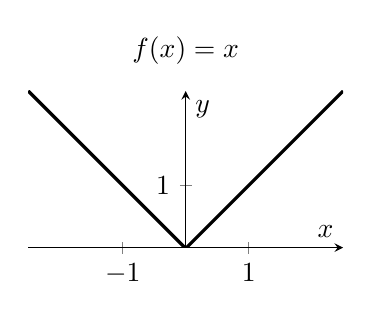
\begin{tikzpicture}
  \begin{axis}[
  axis lines=center, % left, right, box, center, none
  x=8mm,
  y=8mm,
  title={$f(x)=\abs{x}$},
  xlabel=$x$,
  ylabel=$y$,
  xtick={-1,1},
  ytick={1}
  ]
  \addplot[domain=-2.5:2.5, very thick, samples=200] {abs(x)};
\end{axis}
\end{tikzpicture}
\end{figure}

\begin{example}
  Draw the graphs of some elementary functions
  \[
    c, x, x^2, x^3, x^{1/3}, \frac{1}{x}, \frac{1}{x^2}, \sqrt{1-x^2}.
  \]
\end{example}
\begin{example}
  Sketch the graph of $f(x)=1+\sqrt{x-4}$.
\end{example}
\begin{solution}
  Shift the graph of $y=\sqrt{x}$ 1 unit up and 4 units to the right.
\end{solution}
\begin{example}
  Sketch the graph of the function $f(x) = \frac{2-x}{x-1}$.
\end{example}
\begin{solution}
  $f(x) = \frac{2-x}{x-1} = -1 + \frac{1}{x-1}$. So shift the graph of $y=\frac{1}{x}$ 1 unit down and 1 unit to the right.
\end{solution}

\subsection*{Vertical Line Test}
\emph{The graph of a function cannot intersect a vertical line ``$x=\text{\em constant}$'' in more than one point}.

\begin{figure}[H]
  \centering
  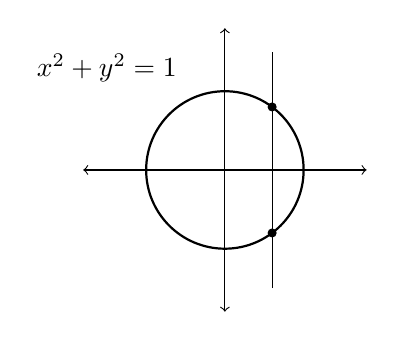
\begin{tikzpicture}
  \draw[<->] (-1.8,0) -- (1.8,0);
  \draw[<->] (0,-1.8) -- (0,1.8);
  \draw[thick] (0,0) circle [radius=1];
  \draw[] (0.6, -1.5) -- (0.6, 1.5);
  \draw[fill, black] (0.6, 0.8) circle [radius=0.05];
  \draw[fill, black] (0.6, -0.8) circle [radius=0.05];
  \node[] at (-1.5, 1.3) {$x^2+y^2=1$};
\end{tikzpicture}
  \caption{The circle $x^2+y^2=1$ is not a graph of a function. It fails the vertical line test.}
\end{figure}

\subsection*{Even and Odd Functions}

\begin{definition}
  We say that $f$ is an \textbf{even function} if $f\left( -x\right) =f\left( x\right) $ for every $x\in D$.
  We say that $f$ is an \textbf{odd function} if $f(-x)=-f(x)$ for every $x\in D$.
\end{definition}

\begin{figure}[H]
  \centering
  \begin{subfigure}{0.3\textwidth}
    \begin{tikzpicture}[scale=2]
  \draw [<->] (-1,0) -- (1,0);
  \draw [<->] (0,-1) -- (0,1);
  \node[below] (X1) at (0.7, 0) {$x$};
  \node[below] (X2) at (-0.7, 0) {$-x$};
  \draw[domain=-1:1] plot (\x, {\x*\x+0.1});
  \draw[dashed] (X1)--(0.7, 0.59);
  \draw[dashed] (X2)--(-0.7, 0.59);
  \draw[dashed] (0.7, 0.59)--(-0.7, 0.59);
  \node[above left] (fx) at (0, 0.59) {$f(x)$};
  \draw[fill] (0, 0.59) circle [radius=.025];
\end{tikzpicture}
    \caption{An even function}
  \end{subfigure}
  \begin{subfigure}{0.3\textwidth}
    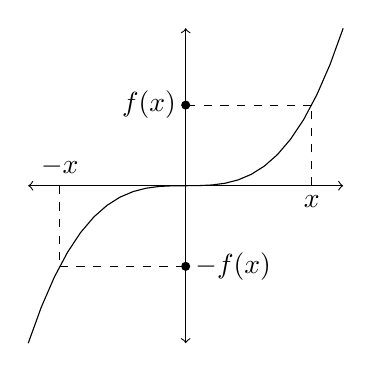
\begin{tikzpicture}[scale=2]
  \draw [<->] (-1,0) -- (1,0);
  \draw [<->] (0,-1) -- (0,1);
  \node[below] (X1) at (0.8, 0) {$x$};
  \node[above] (X2) at (-0.8, 0) {$-x$};
  \draw[domain=-1:1] plot (\x, {\x*\x*\x});
  \draw[dashed] (X1)--(0.8, 0.512);
  \draw[dashed] (X2)--(-0.8, -0.512);
  \draw[dashed] (0.8, 0.512)--(0, 0.512);
  \draw[dashed] (-0.8, -0.512)--(0, -0.512);
  \node[left] at (0, 0.512) {$f(x)$};
  \draw[fill] (0, 0.512) circle [radius=.025];
  \node[right] at (0, -0.512) {$-f(x)$};
  \draw[fill] (0, -0.512) circle [radius=.025];
\end{tikzpicture}
    \caption{An odd function.}
  \end{subfigure}
\end{figure}

Odd functions are symmetric with respect to origin and even functions are symmetric with respect to the $y$-axis.


\begin{example}
  $f(x)=x,f(x)=x^{3}$ are odd and $f(x)=x^{2}$ and $f(x) =x^{4}$ are even and $f(x)=\frac{1}{x+1}$ is neither even or odd.
\end{example}

\begin{example}
  $f(x)=x^{3}+x$ is odd and $f(x)=\frac{1}{x^{2}-1}$ is even and $f(x)=x^{2}+x$
  is either even or odd.
\end{example}

\end{document}
